%\documentclass[12pt,a4paper]{article}
\documentclass[letterpaper,12pt,titlepage]{article}

\usepackage{hyperref}
\usepackage{listings}
\usepackage{wasysym}
\usepackage{graphicx}


\hypersetup{
	colorlinks,
	citecolor=black,
	filecolor=black,
	linkcolor=black,
	urlcolor=black
}

% This is a comment
\title{Software Design Specification and User Interface}
\author{
  \texttt{Sarahi Pelayo (pelayos)}
  \\[.5ex]
  \texttt{Katherine Jeffrey (jeffreyk)}
  \\[.5ex]
  \texttt{Megan Bigelow (bigelowm)}
  \\[.5ex]
  \texttt{Johnathan Lee (leejohna)}
  \\[.5ex]
  \texttt{Jonathan Rohr (rohrj)}
}

\begin{document}
\maketitle

\section{User Interface Prototypes}
\vspace{50pt}
\hspace*{-1in}
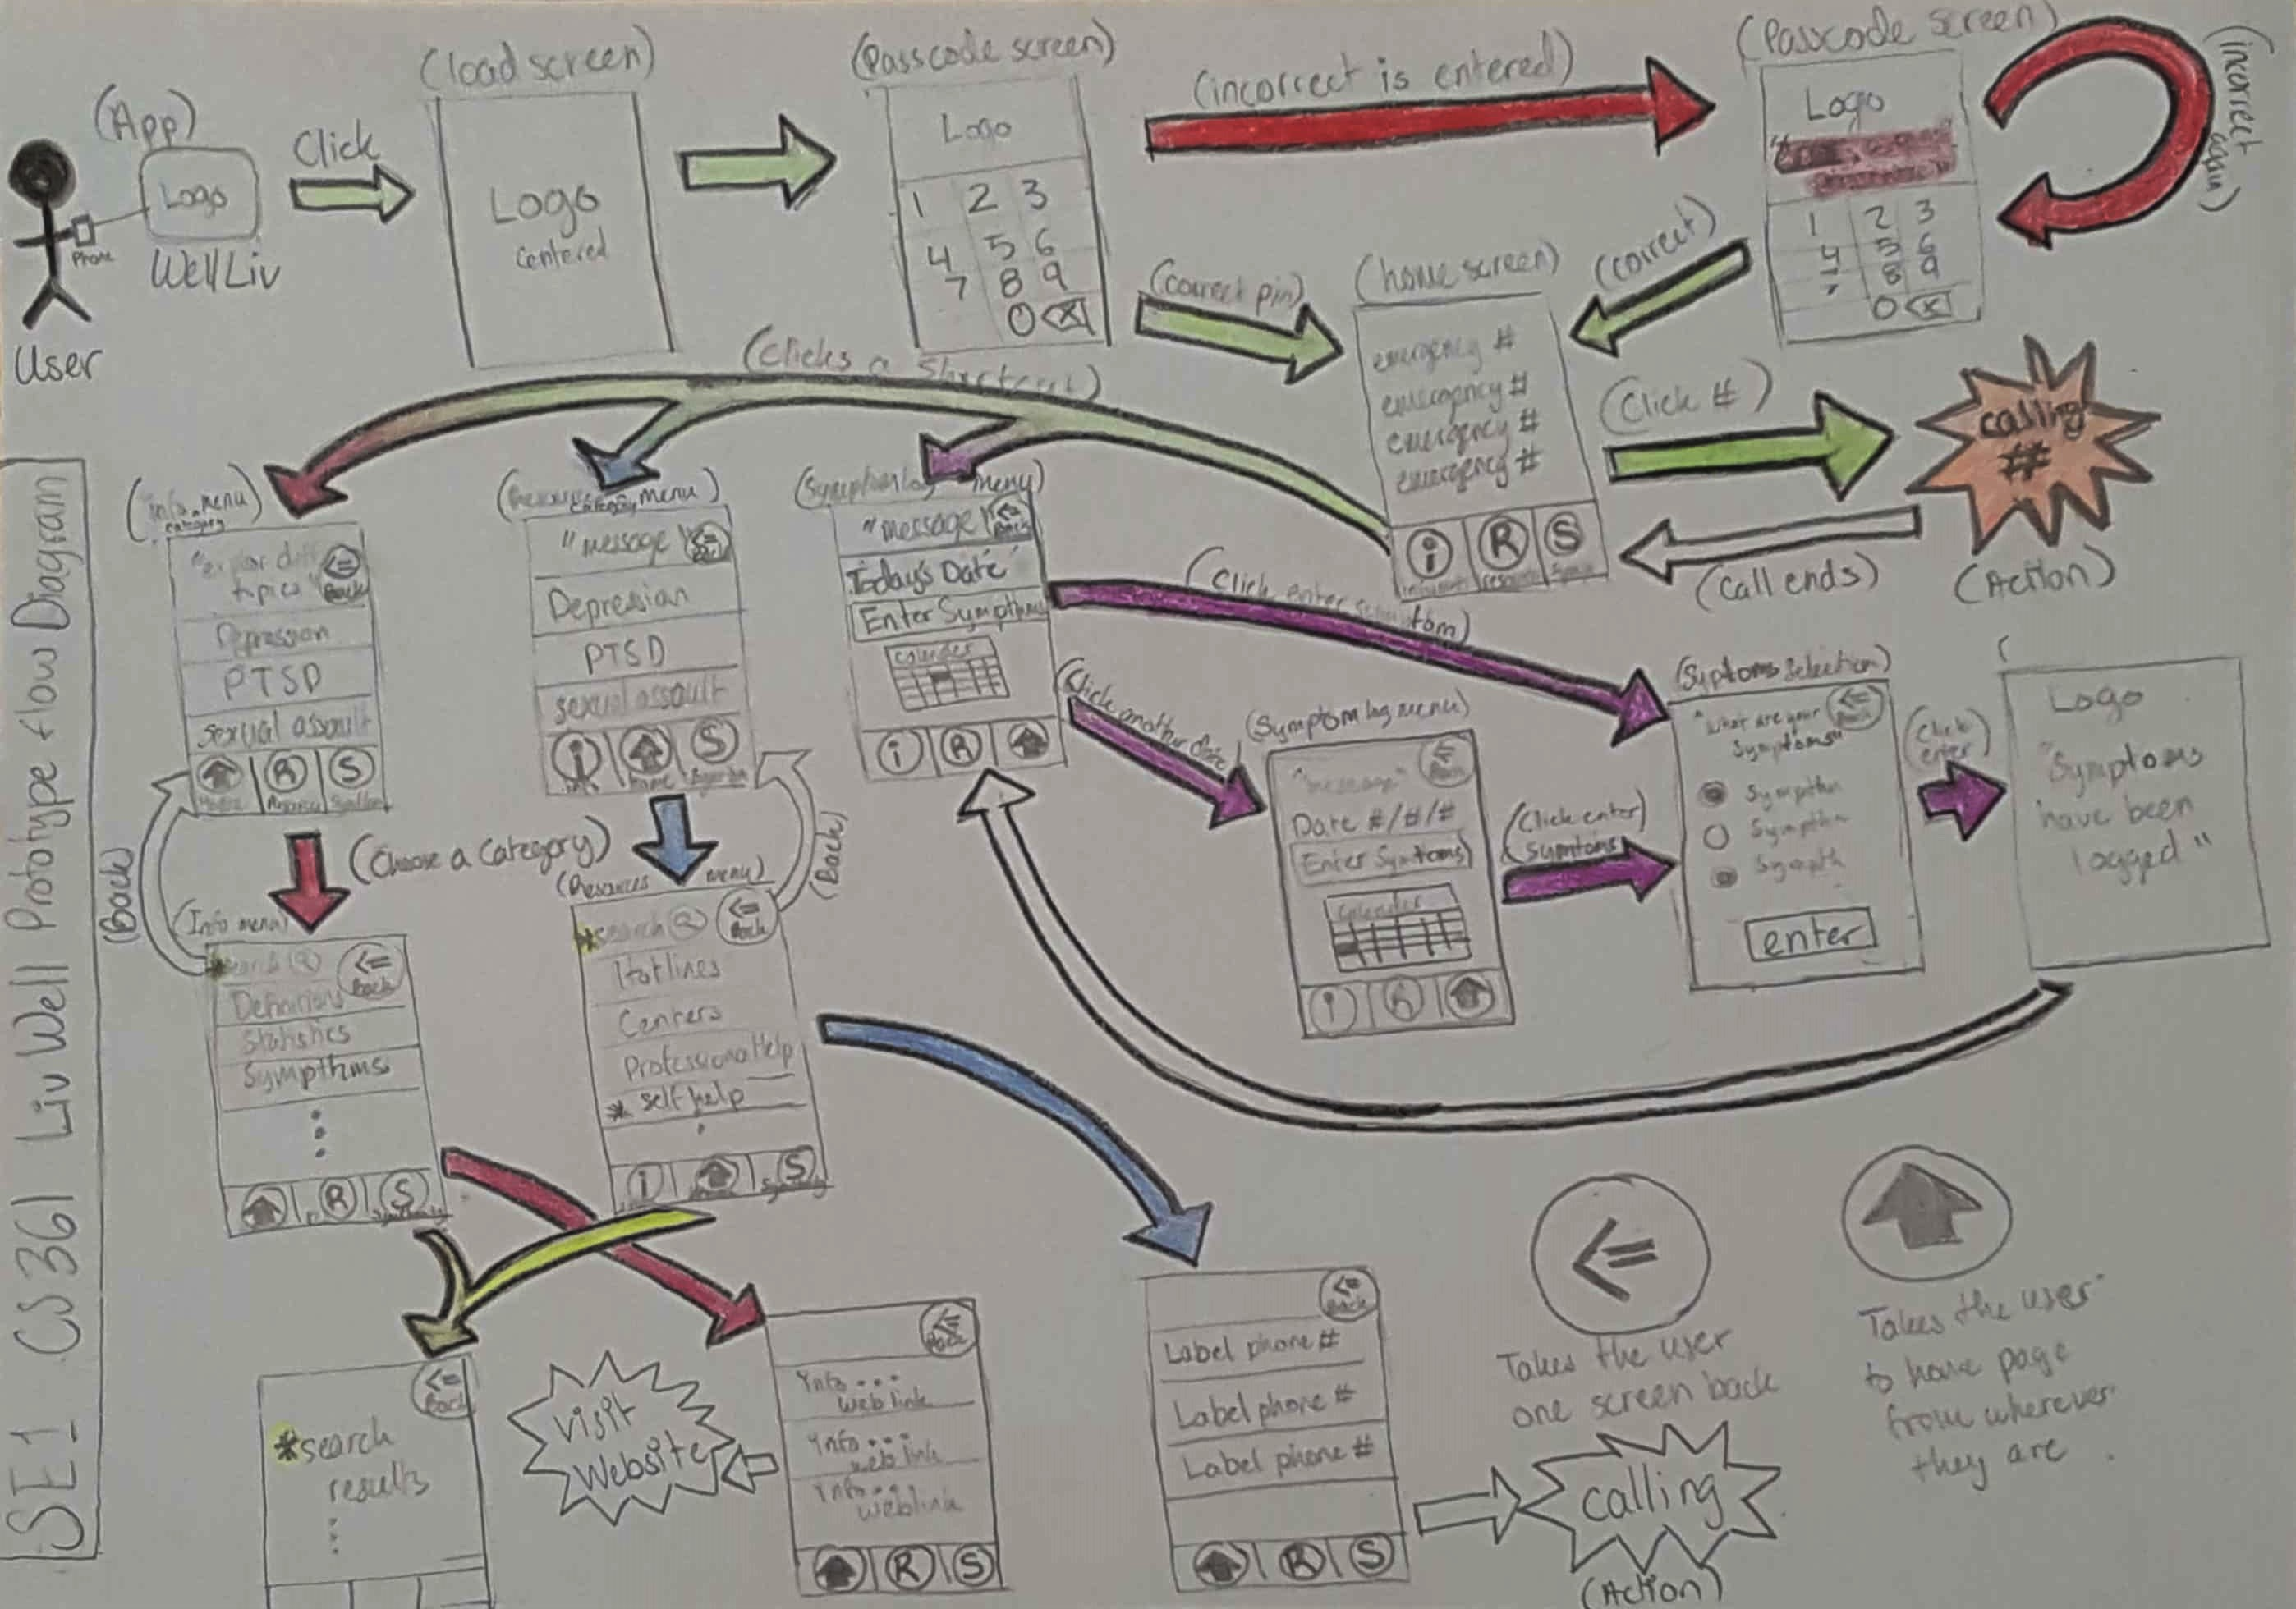
\includegraphics[scale=.25]
{prototype_4}
\newpage
\hspace*{-.2in}
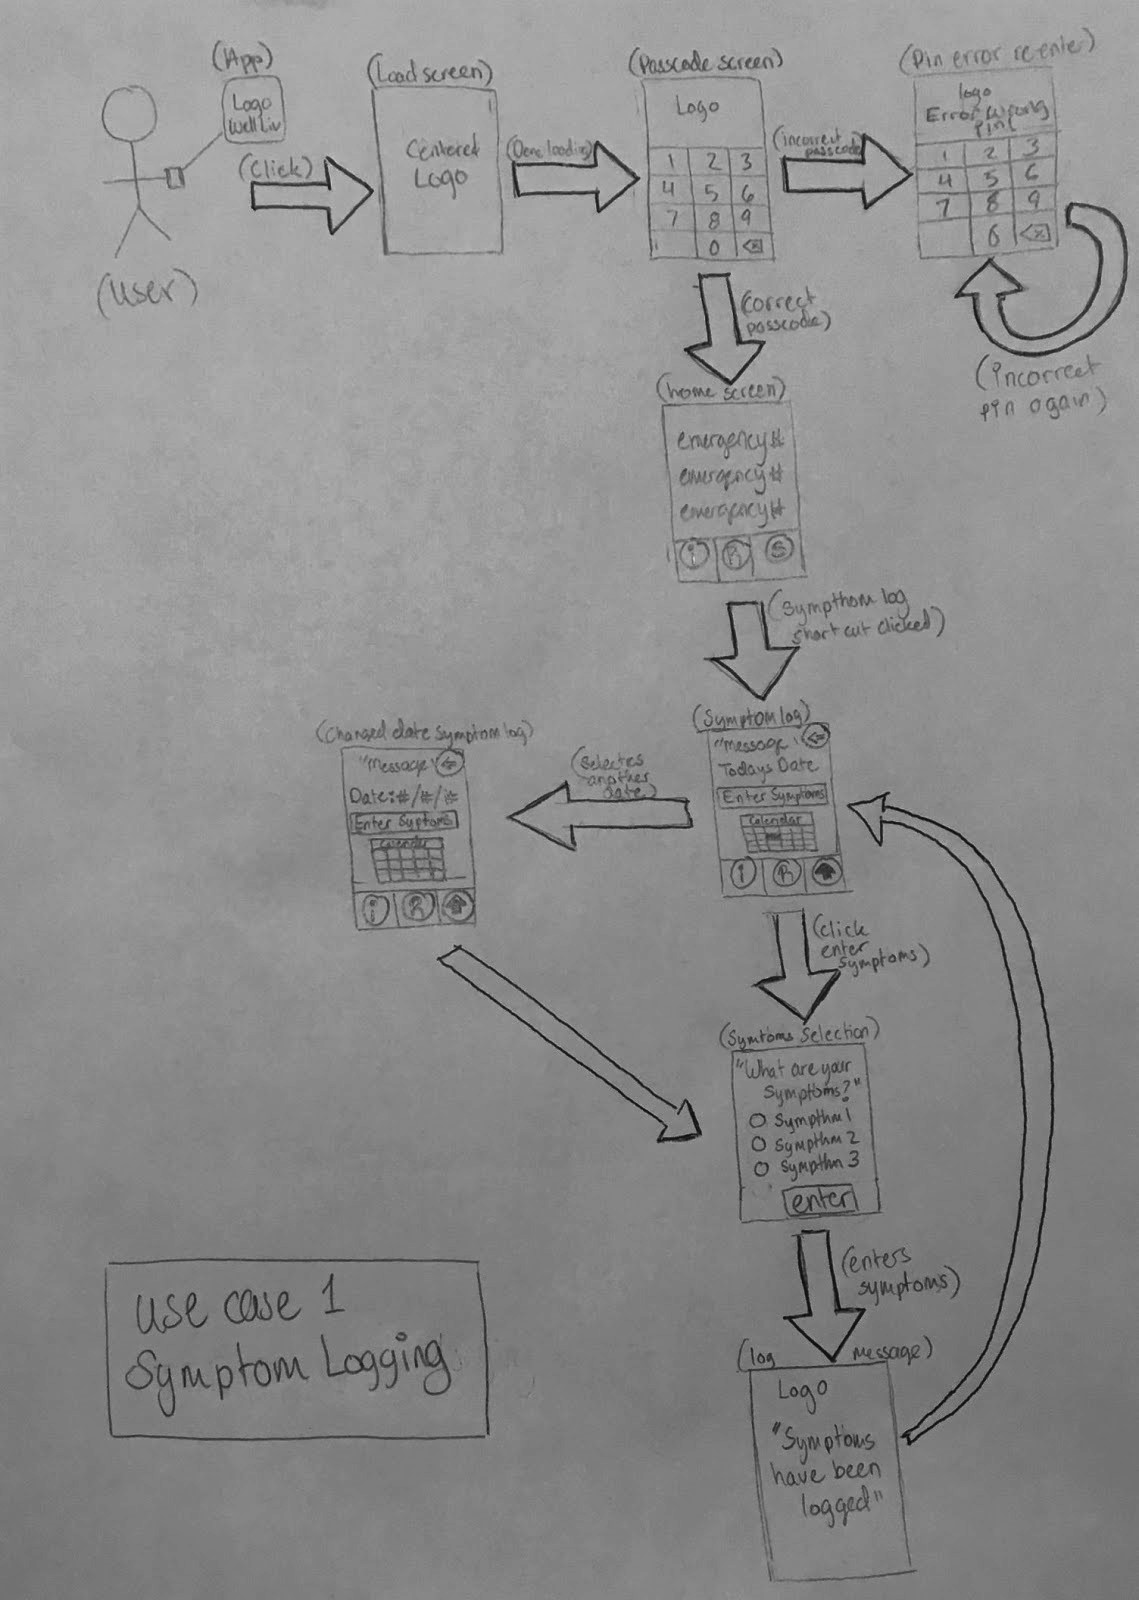
\includegraphics[scale=.45]{prototype_1}
\newpage
\hspace*{-.3in}
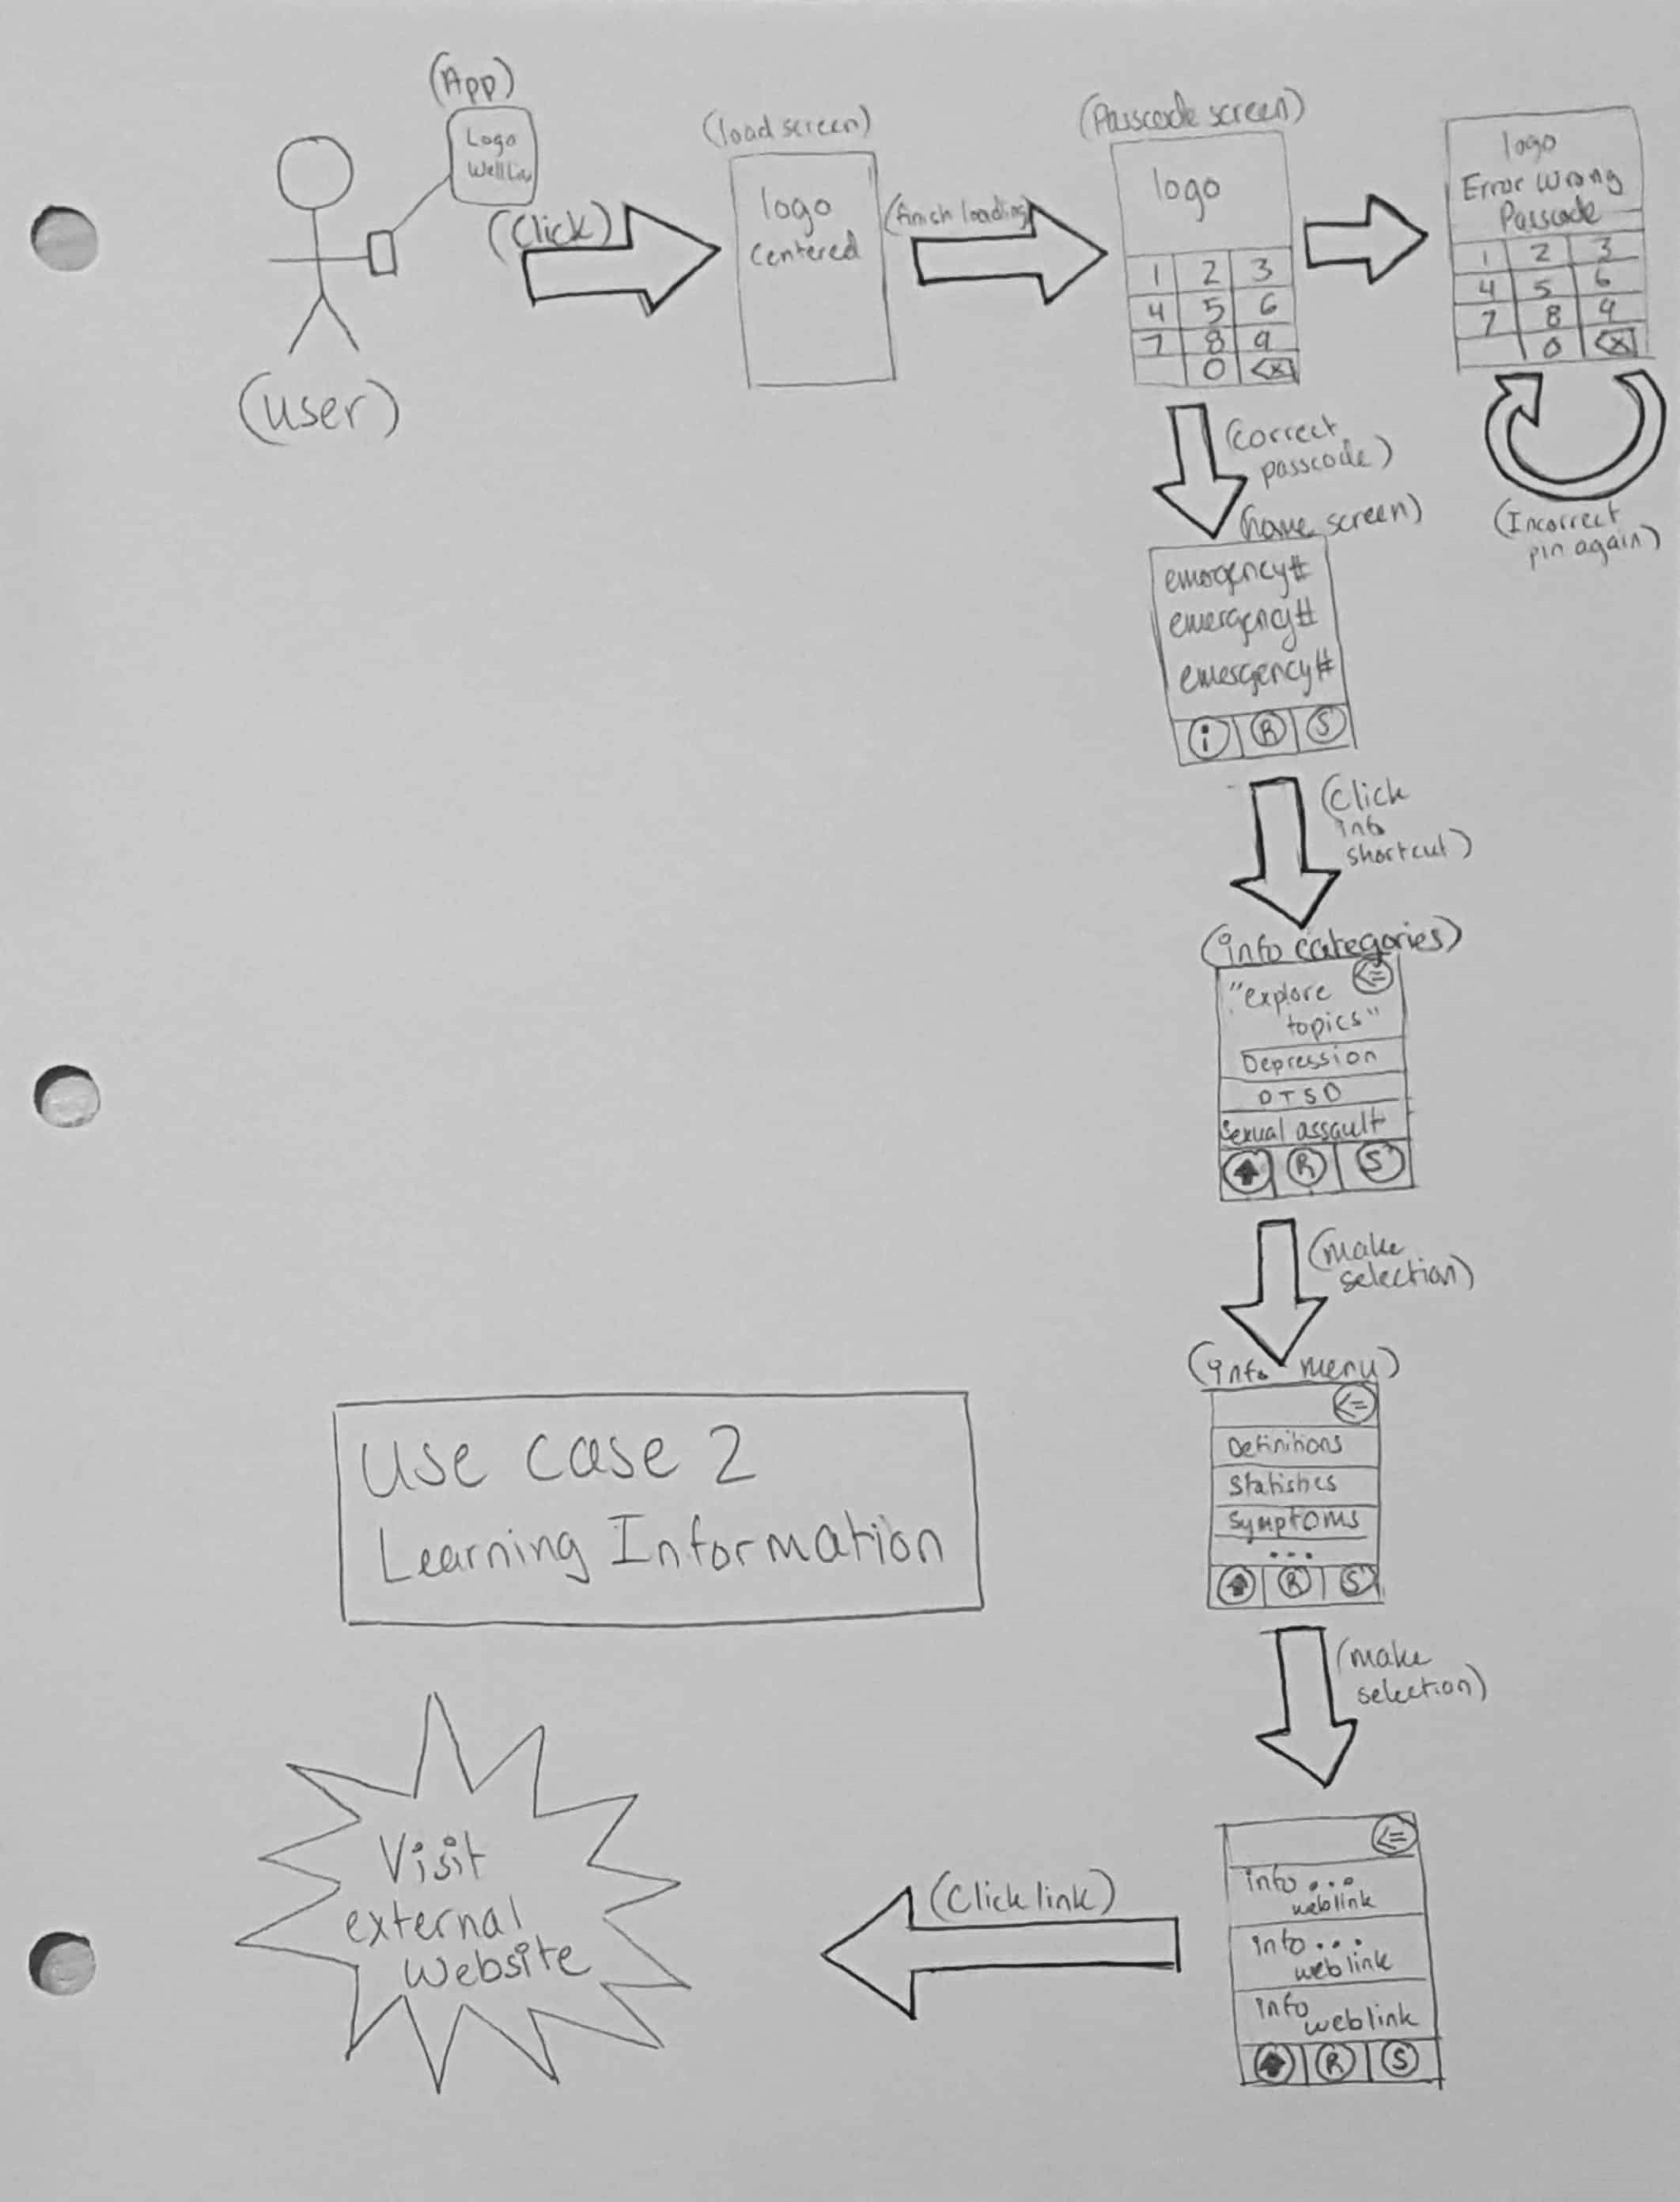
\includegraphics[scale=.25]
{prototype_2}
\newpage
\hspace*{-.3in}
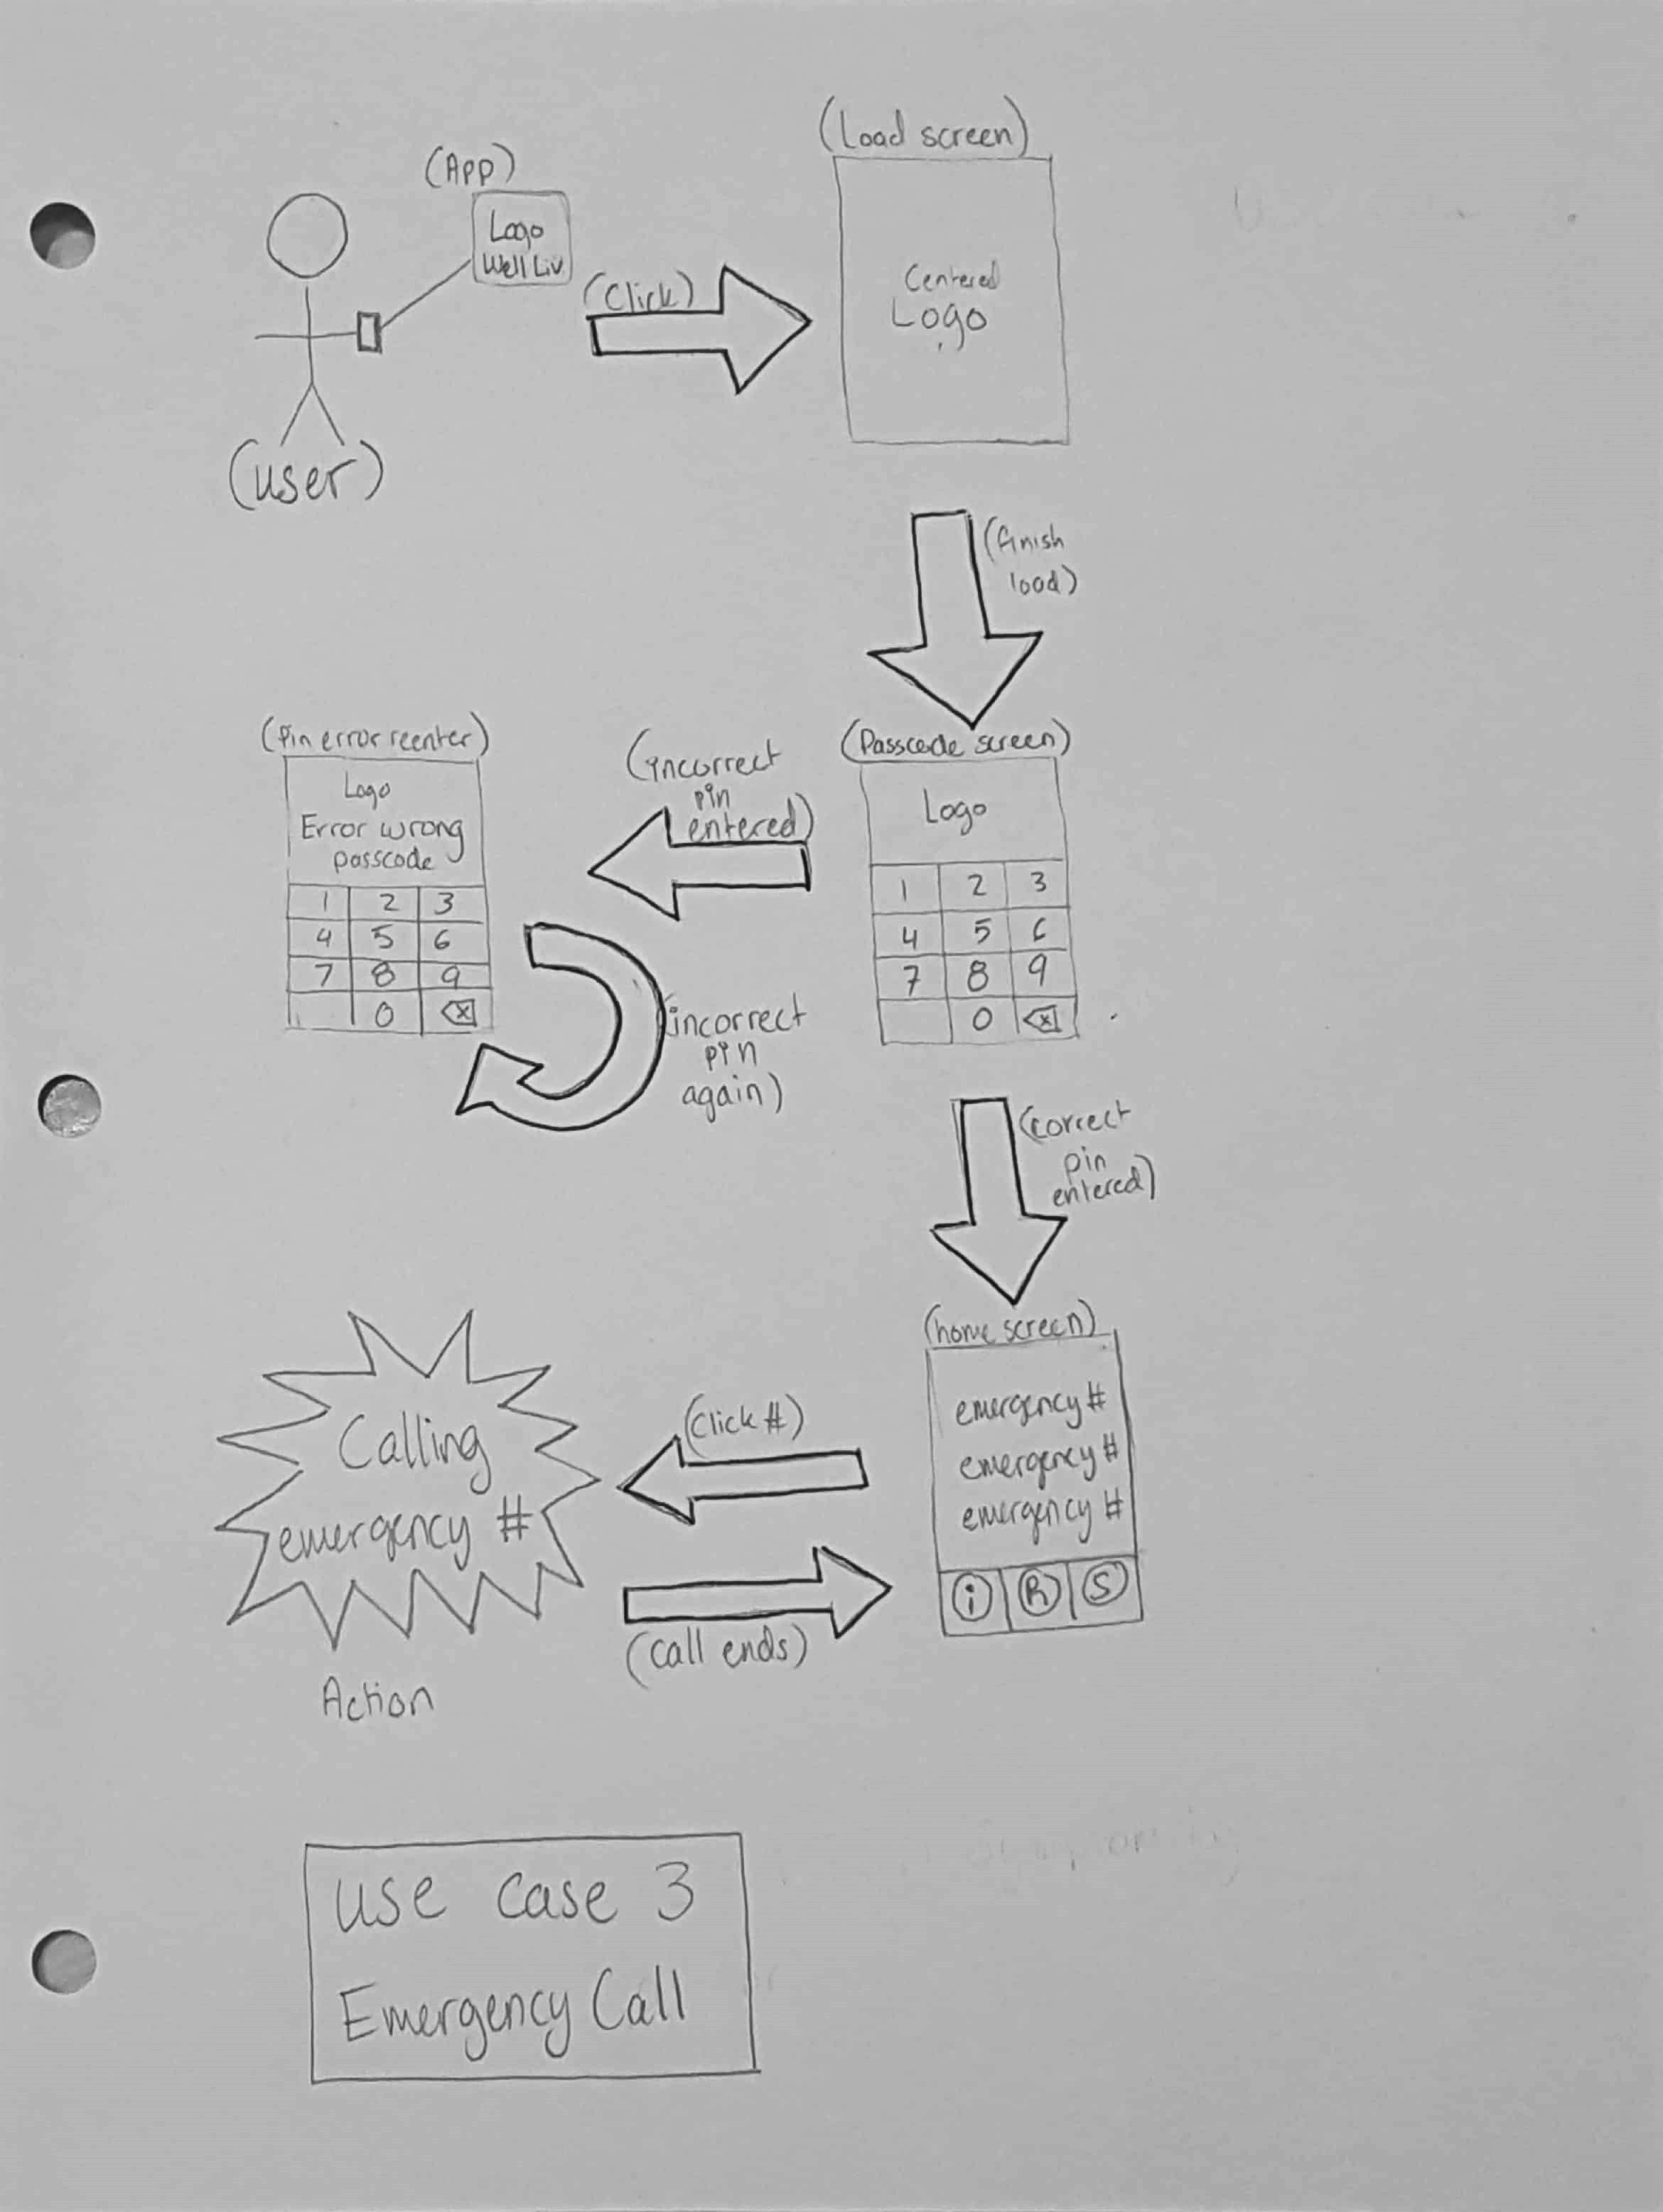
\includegraphics[scale=.22]
{prototype_3}
\newpage
\hspace*{-.2in}
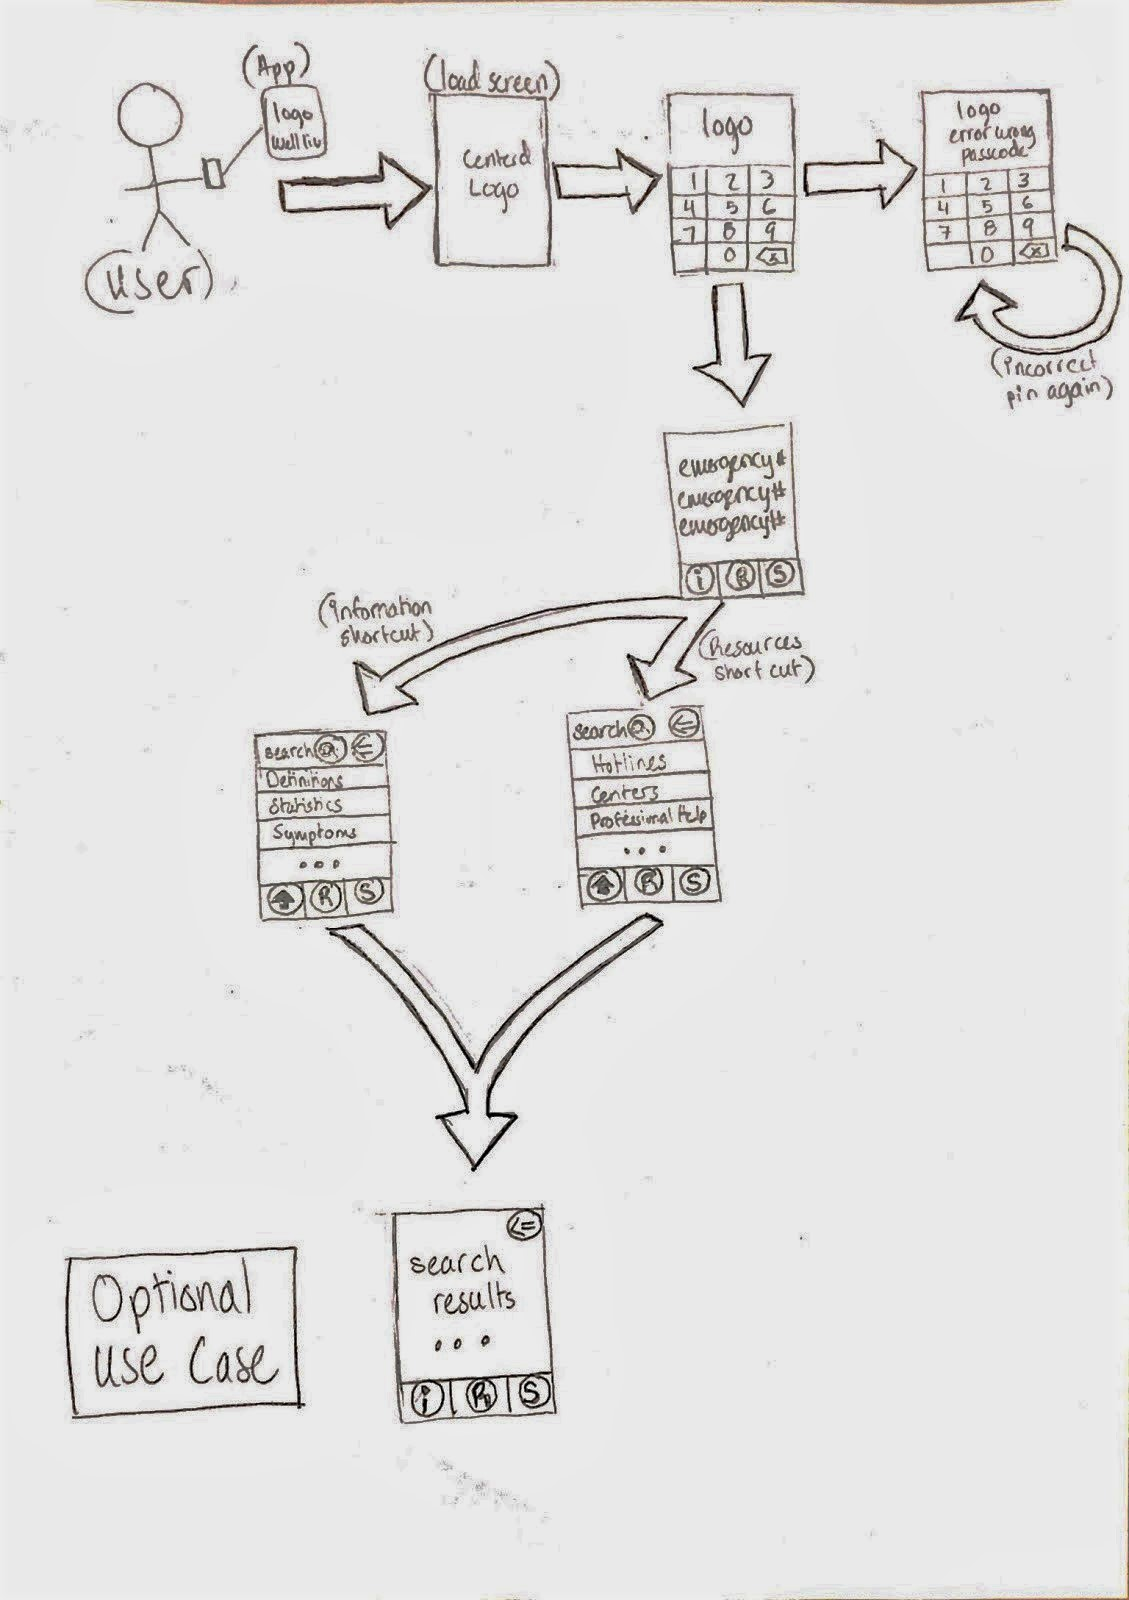
\includegraphics[scale=.44]
{prototype_optional}
\newpage

\noindent
\textbf{Use Case 1:} In this case the user’s goal is to log their symptoms. This begins by the user opening up the application on their phone and entering their passcode to open it up. Once they enter the correct pin they are directed to the home menu. From the home menu they select the symptom log shortcut. The symptom log menu appears with today’s date. They can choose to enter symptoms for the current date or change the date. Once they have the date they want they select enter symptoms. They are presented with a list of different symptoms which they select from and then click enter. They receive a confirmation screen with a message that their symptoms have been logged. Afterward it takes them back to the symptoms log menu.
\newline
\newline
\textbf{Use Case 2: }In this case the user’s goal is to learn new information. This begins by the user opening up the application on their phone and entering their passcode to open it up. Once they enter the correct pin they are directed to the home menu. From the home menu they select the information shortcut. The information category menu appears from which they can select a topic. Once they select their topic they are directed to another menu with options to learn about statistics, definitions, symptoms, and more. Once they decide what type of information they want to explore they are directed to a list with information. The list of information has short information with the website link the infor was sourced from they can then click a link and explore and external website some more.
\newline
\newline
\textbf{Use Case 3:} In this case the user’s goal is to place an emergency call. This begins by the user opening up the application on their phone and entering their passcode to open it up. Once they enter the correct pin they are directed to the home menu. From the home menu they select the number emergency number appropriate to their situation and immediately start dialing where they can get help from the police, poison control, or suicide hotline. After their call ends they land back onto the home page.
\newline
\newline
\textbf{Optional Use Case:} Searching the application for key words the user selects is a feature we hope to implement. The user begins by entering their passcode. Then from the information menu or the resources menu they can then enter text into the search bar. They then get search results they can look through.

\newpage
\section{Class Diagrams}
\vspace{50pt}
\hspace*{-1in}
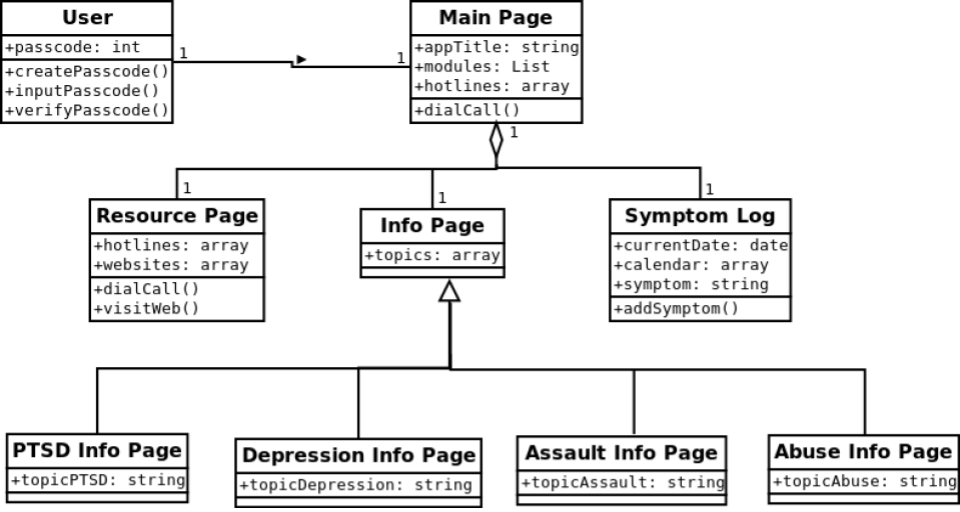
\includegraphics[scale=.55]{UML_Diagram}~\cite{umldia}


\newpage
\section{Sequence Diagrams}
\vspace{50pt}
\hspace*{-1in}
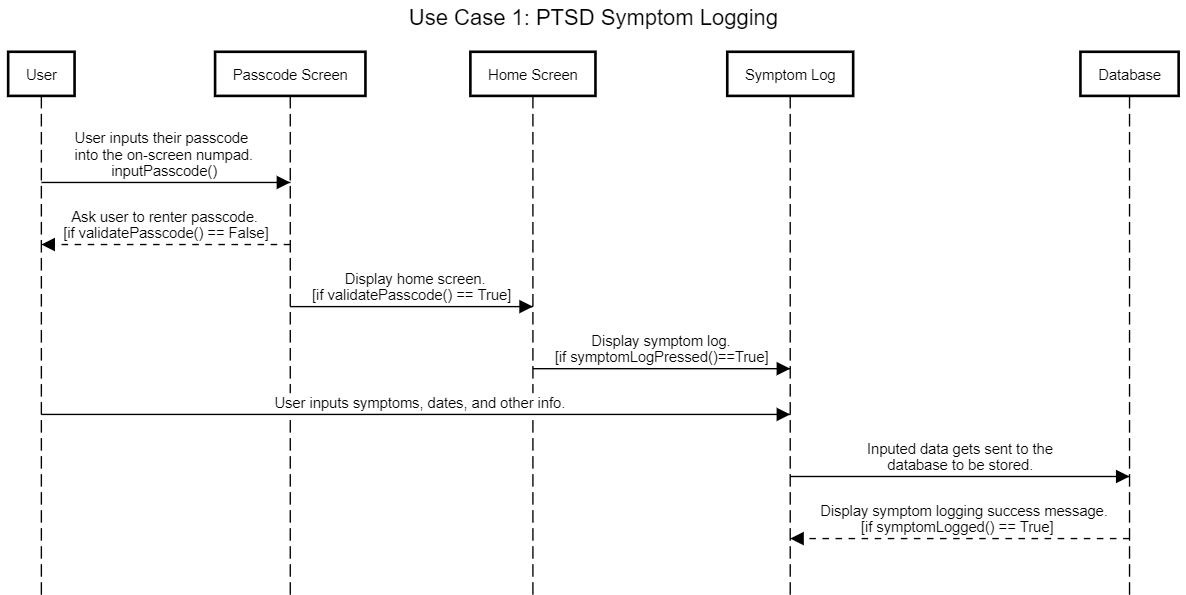
\includegraphics[scale=.44]{Use_Case_1__PTSD_Symptom_Logging}~\cite{seqdia}
\newpage
\hspace*{-1.2in}
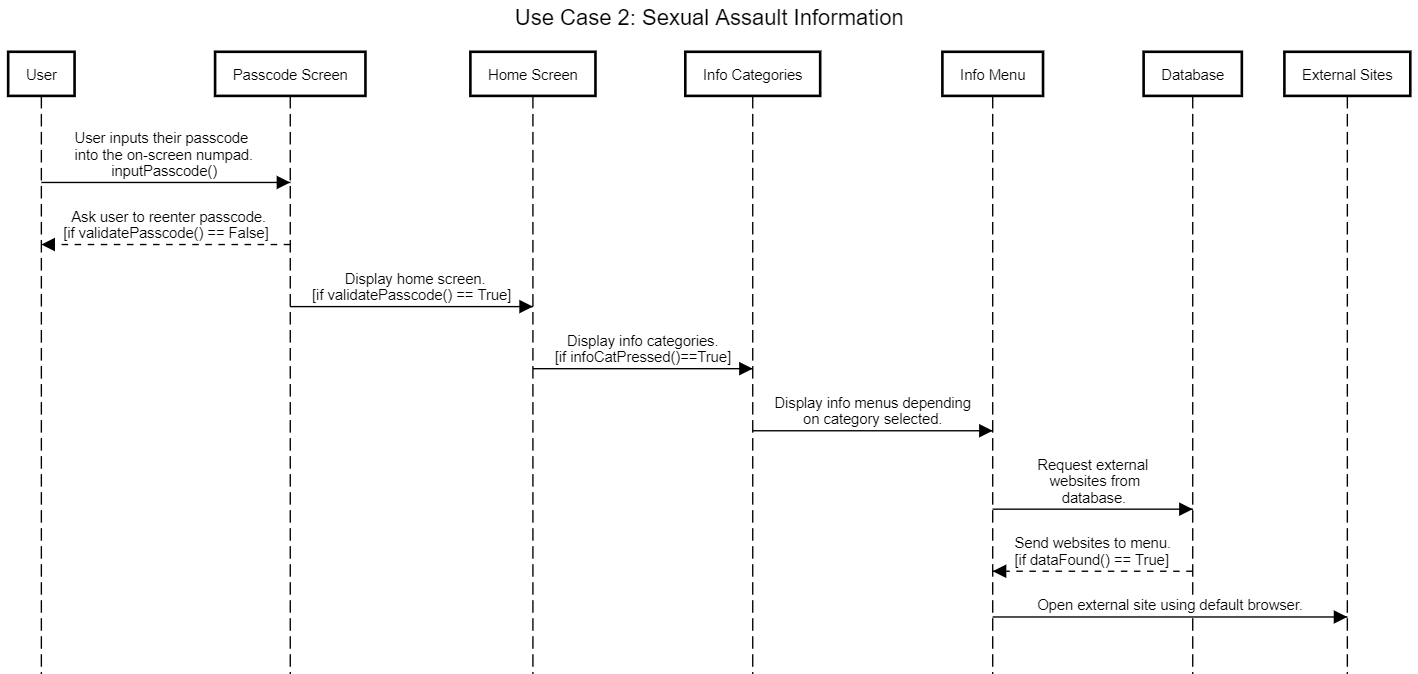
\includegraphics[scale=.38]{Use_Case_2__Sexual_Assault_Information}
\newpage
\hspace*{-1.2in}
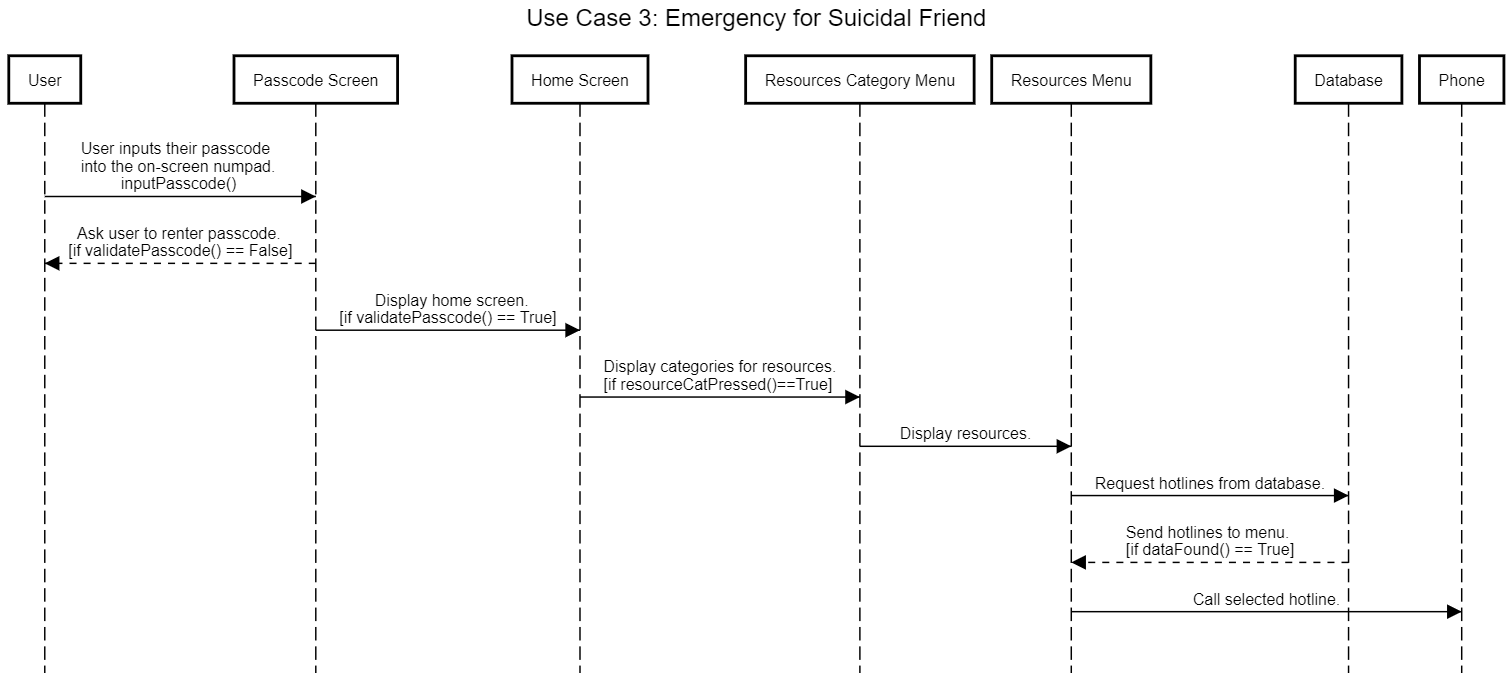
\includegraphics[scale=.36]{Use_Case_3__Emergency_for_Suicidal_Friend}
\vspace{0pt}
\section{Meeting Report}
\underline{Third meeting:} 2/1 in person after class, 5:50pm-6:10pm
\begin{itemize}
\item Members present: Sarahi Pelayo, Katherine Jeffrey, Jonathan Rohr, Johnathan Lee, Megan Bigelow
\item Discussed: Verification of sources researched 
\item Progress: Sarahi make a paper low level prototype of all the screens the user will see and the flow between them. Jonathan has selected to research PTSD. Johnathan has selected to research sexual assault. Katherine has chosen to research abuse and shared links and a phone number to a crisis text line. Megan chose the topic of depression.
\item Plans: Work on assignment 3. Sarahi will break current paper prototype into the three use cases. Research the software we want to use for the UML diagrams. Work on the sequence diagram. 
\item Customers were willing and able to meet 
\end{itemize}
\newpage
\noindent
\underline{Date:} 2/5 in KEC, 4pm-5pm
\begin{itemize}
\item Progress: Finished sequence diagrams, UML class diagram, and the user interface prototypes. Worked on the basic visual layout of the application on Android Studio. Completed some research on the information we will have in the application.
\end{itemize}

\noindent
\textbf{Next Week}
\newline
\newline
Plans and goals:
\begin{itemize}
\item Learn how to code in Java and use the Android Studio interface.
\item Learn how databases work and how to implement them.
\item Finish up any remaining research.
\item Start implementing basic code
\end{itemize}
\newpage

\bibliography{myref}
\bibliographystyle{ieeetr}

\end{document}